\documentclass{article}
\usepackage{amsmath}
\usepackage{amssymb}
\usepackage{amsfonts}
\usepackage{inputenc}
\usepackage{graphicx}
\usepackage{systeme}
\title{Geometria e Algebra}
\begin{document}
\section{Geometria affine (richiami)}
\begin{flushleft}
	In geometria useremo dei spazi in cui lavoreremo che sono: retta, piano e spazio
\end{flushleft}
\begin{itemize}
	\item retta (euclidea) affine $(A^1)$
	\item piano affine ($\pi$ = piano) ($A^2$) $\pi \supseteq r$
	      \begin{flushleft}
		      $r_1$ e $r_2$ rette in $\pi$ sono:
	      \end{flushleft}
	      \begin{itemize}
		      \item inicidenti se $r_1 \cap r_2=\{ P \}$ (p punto)
		      \item parallele se $r_1 \cap r_2=\emptyset$ e se $ r_1 =r_2$
	      \end{itemize}
	\item spazio affine
	      \begin{flushleft}
		      I suoi sottoinsiemi notevoli sono:
	      \end{flushleft}
	      \begin{itemize}
		      \item punti (P)
		      \item rette (r)
		      \item piani ($\pi$)
	      \end{itemize}
	      \begin{flushleft}
		      Ora le varie regole
	      \end{flushleft}
	      \begin{itemize}
		      \item $\pi$ e $\pi$' nello spazio sono:
		            \begin{itemize}
			            \item incidenti se $\pi \cap \pi ' =r$
			            \item paralleli se $\pi \cap \pi ' =\emptyset$ e se $\pi = \pi '$
		            \end{itemize}
		      \item r e $\pi$ nello spazio sono:
		            \begin{itemize}
			            \item incidenti se $\pi \cap r = \{ P \}$
			            \item paralleli se $\pi \cap r = \emptyset$ e se $r \subseteq \pi$
		            \end{itemize}
		      \item r e r' sono:
		            \begin{itemize}
			            \item complanari se $\exists \pi: \quad \pi \subseteq r \land \pi \subseteq r'$
			            \item sgherbe se $r \cap r' = \emptyset$ e se $r \nparallel r'$
		            \end{itemize}
	      \end{itemize}
\end{itemize}

\section{Vettori orientati}
\begin{flushleft}
	I vettori orientati sono segmenti che partono da un punto di origine O e arrivano ad un punto P, se si vogliono avere piu' vettori
	questi devono partire tutti dallos stesso punto O
\end{flushleft}
\begin{flushleft}
	Def: Esiste una funzione $\Phi_o : A_o \rightarrow V_o^{1/2/3}$
\end{flushleft}
\begin{equation*}
	\Phi_o(P)=\overrightarrow{OP}
\end{equation*}
\begin{flushleft}
	Nota: La funzione $\Phi_o$ e' biettiva
\end{flushleft}
\subsection{Somma tra vettori}
\begin{flushleft}
	Def:$\forall v = \overrightarrow{OP}$ e $v' = \overrightarrow{OP}' in V_o^{1/2/3} \to \exists ! v''=\overrightarrow{OP}''$
\end{flushleft}
\begin{flushleft}
	Per la somma tra vettori si costruisce un parallelogramma con le parallele di entrambi i vettori di cui si intende sommare
	e poi si traccia una diagonale dal punto O fino al vertice che si formera e questa diagonale rappresentera' la somma di 2 vetttori
\end{flushleft}
\subsection{Proprieta' della somma in $V_o^{1/2/3}$}
\begin{enumerate}
	\item La somma e' associativa
	\item $\exists \overrightarrow{OO} \in V_o^{1/2/3}$ e' un elemento neutro della somma
	\item $\forall \overrightarrow{OP}, \exists \overrightarrow{OP}' \in V_o^{1/2/3}$ tale che
	      \begin{equation*}
		      \overrightarrow{OP} +\overrightarrow{OP}' = \overrightarrow{OO}=\overrightarrow{OP}' +\overrightarrow{OP}
	      \end{equation*}
	\item La somma e' commutativa
\end{enumerate}
\section{Moltiplicazione dello scalare}
\begin{flushleft}
	Def: $\forall v = \overrightarrow{OP} \in V_o^n$ (n=1,2,3)
	$\forall t \in \mathbb{R}, \exists !t: v=t*\overrightarrow{OP} \in V^n_o$ tale che
	$t*\overrightarrow{OP}=\overrightarrow{OP_t}$ dove $P_t \in A^t$ e' dato da
\end{flushleft}
\begin{itemize}
	\item Se $t=0$ $\to$ $P_t:= 0 \to t*\overrightarrow{OP}=\overrightarrow{OO}$
	\item Se $t>0$ $\to$ $P_t$ e' nella retta di $\overrightarrow{OP}$:
	      \begin{equation*}
		      \frac{lungh(\overrightarrow{OP_t})}{lungh(\overrightarrow{OP})} = t = |t|
	      \end{equation*}
	\item Se $t<0$:
	      \begin{equation*}
		      \frac{lungh(\overrightarrow{OP_t})}{lungh(\overrightarrow{OP})} = -t = |t|
	      \end{equation*}
\end{itemize}
\begin{flushleft}
	Tutto questo e' vero se $\overrightarrow{OP} \neq \overrightarrow{OO}$
	se invece $\overrightarrow{OP} = \overrightarrow{OO}$ allora $t*\overrightarrow{OO}=\overrightarrow{OO}$
\end{flushleft}
\begin{flushleft}
	Quindi esiste una funzione:
\end{flushleft}
\begin{itemize}
	\item $\mathbb{R}xV_o^n \to V_o^n$
	\item $(t,v) \to t*v$
\end{itemize}
\subsection{Proprieta' della moltiplicazione}
\begin{flushleft}
	$\forall v',v'' \in V_o^n$\\
	$\forall t',t'' \in \mathbb{R}$
\end{flushleft}
\begin{enumerate}
	\item $t' * (t''*v)=(t''*t')*v$
	\item $1*v=v$
	\item $t' + (t''+v)=(t''+t')+v$
	\item $t*(v'+v'')=(t*v')+(t*v'')$
\end{enumerate}
\section{Riferimenti affini e coordinate}
\subsection*{[n=1]}
\begin{flushleft}
	Fisso $O \in A^n$ e fisso $\overrightarrow{i} \in V^n_O$, con $\overrightarrow{i} \neq \overrightarrow{OO}$
\end{flushleft}
\begin{flushleft}
	Allora $ \forall v = \overrightarrow{OP} \in V^1_O,\exists ! x\in \mathbb{R}:v= \overrightarrow{OP} = x* \overrightarrow{i}$
\end{flushleft}
Quindi
\begin{equation*}
	|x|=\frac{lungh(\overrightarrow{OP})}{lungh(\overrightarrow{i})}
\end{equation*}
\begin{flushleft}
	Tale x si dice coordinata di $\overrightarrow{OP}$ (o del punto P) e il vettore di riferimento affine e' $(o;\overrightarrow{i})$
\end{flushleft}
\begin{flushleft}
	il segno di x dipende da dove si trova il vettore OP rispetto ad il vettore i
\end{flushleft}
\begin{itemize}
	\item + se si trova nella stessa parte del vettore di OP
	\item - se si trova nella parte opposta del vettore di OP
\end{itemize}
\subsection*{[n=2]}
\begin{flushleft}
	Fisso $O \in A^2$ e fisso $\overrightarrow{i},\overrightarrow{j} \in V^2_O$, con $\overrightarrow{i},\overrightarrow{j}$ non multipli tra di loro
\end{flushleft}
\begin{equation*}
	V_O^2 \iff \mathbb{R}^2
\end{equation*}
\begin{equation*}
	(x,\overrightarrow{i})+(y,\overrightarrow{j}) \leftarrow (x,y)
\end{equation*}
\begin{flushleft}
	Allora $\forall \overrightarrow{v}=\overrightarrow{OP} \in V^2_O \quad \exists ! (x,y) \in \mathbb{R}^2$ tale che
\end{flushleft}
\begin{equation*}
	\overrightarrow{v}=\overrightarrow{OP}=(x,\overrightarrow{i})+(y,\overrightarrow{j})
\end{equation*}
\subsection*{[n=3]}
\begin{flushleft}
	Fisso $O \in A^3$ e fisso $\overrightarrow{i},\overrightarrow{j},\overrightarrow{k} \in V^3_O$
\end{flushleft}
\begin{equation*}
	V_O^3 \iff \mathbb{R}^3
\end{equation*}
\begin{equation*}
	x*\overrightarrow{i}+y*\overrightarrow{j}+z*\overrightarrow{k} \leftarrow (x,y,z)
\end{equation*}
\begin{flushleft}
	$\overrightarrow{i},\overrightarrow{j},\overrightarrow{k}$ non devono essere complanari
\end{flushleft}
\begin{flushleft}
	Def: (x,y,z) sono coordinate di $v=\overrightarrow{OP}$ (o di P)
\end{flushleft}
quindi possiamo dedurre questo
\begin{equation*}
	\mathbb{R}^n \iff V_O^n
\end{equation*}
\section{Equazioni vettoriali di rette e piani}
\begin{flushleft}
	L'equazione vettoriale di una retta r,
	$(O,\overrightarrow{i},\overrightarrow{j},\overrightarrow{k})$ e' riferimento affine (in $A^2,A^3$)
\end{flushleft}
\begin{flushleft}
	$\exists ! r_0 : r_0 || r, O \in r_0$
\end{flushleft}
\begin{flushleft}
	$ Q \in r_0, Q \neq O, \overrightarrow{v_2}=\overrightarrow{OQ} \quad (\neq \overrightarrow{OO})$
\end{flushleft}
\begin{flushleft}
	$\forall P \in A^{2/3}$ si ha $ P \in r$ e $P_0 \neq P \iff \overline{P_0 P} || r_0 \quad \exists ! P' \in r_0$
\end{flushleft}
\begin{flushleft}
	$\to \overrightarrow{OP} = \overrightarrow{OP_0} + \overrightarrow{OP'} (\in V_0^{2/3})$
\end{flushleft}
\begin{itemize}
	\item $\overrightarrow{OP}$ = il valore e' variabile
	\item $\overrightarrow{OP_0}$ = il valore e' fisso
	\item $\overrightarrow{OP'}$ = il valore e' variabile
\end{itemize}
\begin{flushleft}
	$\overrightarrow{OP'}$ e' sulla retta $r_0$ che ha riferimento affine $(O;\overrightarrow{v_r})$
\end{flushleft}
\subsection*{Equazione vettoriale di una retta}
\begin{equation*}
	r = \{ P \in A^{2/3} | \exists t \in \mathbb{R}: \overrightarrow{OP}=\overrightarrow{OP_0}+t*\overrightarrow{v_r} \}
\end{equation*}
\begin{flushleft}
	Def:  $\overrightarrow{v_r}$ si dice vettore direttore
\end{flushleft}
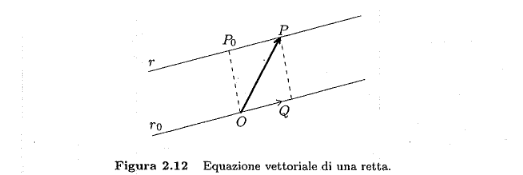
\includegraphics[bb=0 0 350 100]{equazione-retta-v.png}
\subsection*{Equazione vettoriale per piani}
\begin{flushleft}
	$\forall \overrightarrow{v} \in V^3_0, \exists ! (s,t,d):
		s\overrightarrow{i} + t\overrightarrow{j} + d\overrightarrow{k} = \overrightarrow{r}$
\end{flushleft}
\begin{flushleft}
	questi vettori non devono essere complanari
\end{flushleft}
\begin{flushleft}
	$ \exists \pi_0 :\pi_0 || \pi \land O \in  \pi_0$
\end{flushleft}
\begin{equation*}
	P\in \pi \iff \overrightarrow{OP'} \subseteq \pi_0 \iff \overrightarrow{OP'}=\overrightarrow{OP} - \overrightarrow{OP_0} \quad \in V^2_0
\end{equation*}
\subsubsection*{Equazione vettoriale di $\pi$}
\begin{equation*}
	\exists ! (s,t) \in \mathbb{R}^2:\overrightarrow{OP}=\overrightarrow{OP_0}+s\overrightarrow{v}+t\overrightarrow{w}
\end{equation*}

\section{Campi}
\begin{flushleft}
	Def: Campi sono insiemi di numeri in cui si fanno operazioni
\end{flushleft}
\begin{flushleft}
	K e' un campo se e' un insieme con 2 operazioni
\end{flushleft}
\begin{itemize}
	\item + : $KxK \to K$
	\item * : $KxK \to K$
\end{itemize}
\subsection{Somma nei campi}
\begin{enumerate}
	\item La somma e' assiciativa
	\item $\exists O_k \in \mathbb{K} : x+O_k=x \quad \forall x\in \mathbb{K}$
	\item $\forall x \in  \mathbb{K},\exists (-x) \in \mathbb{K}:x+(-x)=O_k$
	\item x+y=y+x $\forall x,y \in \mathbb{K}$
\end{enumerate}
\subsection{Prodotto nei campi}
\begin{enumerate}
	\item Il prodotto e' assiciativa
	\item $\exists 1_k \in \mathbb{K} : x*1_k=x \quad \forall x\in \mathbb{K}$
	\item $\forall x \in  \mathbb{K},\exists x^{-1} \in \mathbb{K}:x*x^{-1}=1_k$
	\item x+y=y+x $\forall x,y \in \mathbb{K}$
\end{enumerate}
\begin{itemize}
	\item D $\rightarrow$ x*(y+z)=(x*y)+(x*z)
	\item D $\leftarrow$ (x+y)*z)=(z*y)+(x*z)
\end{itemize}
\subsection*{Esempi}
\begin{enumerate}
	\item $\mathbb{N}:$ no , $\mathbb{Z}: $ no
	\item $\mathbb{Q}:$ si, $\mathbb{R}: $ si
	\item $\mathbb{Z}_n$ e' un campo se e soltanto se se n e' un numero primo
\end{enumerate}
\section{Spazi Vettoriali}
\begin{flushleft}
	Def: spazio veottoriale su K e' un insieme V con 2 funzioni:
\end{flushleft}
\begin{itemize}
	\item +: $VxV \to V \quad \quad (v',v'') \to v' + v''$
	\item *: $KxV \to V \quad \quad (k,v)\to kv$
\end{itemize}
\subsection*{Proprieta'}
\subsubsection*{Somma}
\begin{enumerate}
	\item Associativa $\forall v,w,u \in \mathbb{V}$
	\item $\exists O_v \in V: $ elemento neutro $\forall v \in \mathbb{V}$
	\item $\forall v \in  \mathbb{V},\exists (-v) \in \mathbb{V}:v+(-v)=O_v$
	\item v+w=w+v $\quad \forall v,w \in \mathbb{V}$
\end{enumerate}
\subsubsection*{Prodotto}
\begin{enumerate}
	\item Associativa $\forall v,w,u \in \mathbb{V}$
	\item $\exists 1_v \in V: $ elemento neutro $\forall v \in \mathbb{V}$
	\item $\forall v \in  \mathbb{V},\exists v^{-1} \in \mathbb{V}:v+v^{-1}=O_v$
	\item v*w=w*v $\quad \forall v,w \in \mathbb{V}$
\end{enumerate}
\begin{itemize}
	\item $k*(v_1+v_2)=(k*v_1)+(k*v_2) \quad \quad \forall v_1,v_2 \in \mathbb{V}, \forall k \in \mathbb{K}$
	\item $v*(k_1+k_2)=(v*k_1)+(v*k_2) \quad \quad \forall k_1,k_2 \in \mathbb{K}, \forall v \in \mathbb{V}$
\end{itemize}
\begin{flushleft}
	Def: $\forall$ spazio vettoriale V (su K) e' un sotto spazio di V e' un sottoinsieme
\end{flushleft}
\begin{flushleft}
	Un $W \subseteq V$ e' sottospazio (vettoriale) se:
\end{flushleft}
\begin{equation*}
	W+W \subseteq W \quad K*W \subseteq W \quad W \neq \emptyset
\end{equation*}
\begin{flushleft}
	($W\leq V$) e' un rafforzamento di $\subseteq$
\end{flushleft}
\subsubsection*{Lemma:}
\begin{flushleft}
	Se V e' un sottospazio vettoriale e $W \leq V$ allora $W$ e' uno spazio vettoriale con somma e prodotto dati da quelli di V ristretti ai vettori di $W$
\end{flushleft}
\textbf{Esempi:}
\begin{enumerate}
	\item $Der(a,b)=\{ f \in \mathbb{R}^{(a,b)} | \text{ f e' derivabile } \}$
	\item $C^0(a,b)= \{ f \in \mathbb{R}^{(a,b)} | \text{ f e' continua } \}$
	      \begin{equation*}
		      Der(a.b) \subseteq C^0(a,b) \land Der(a,b) \leq C^0(a,b)
	      \end{equation*}
	\item $Conv(\mathbb{R}^{\mathbb{N}}) = \{ \{a\}_n | \exists \text{ limite $\in \mathbb{R}$ (convergente)}\}$
	      \begin{flushleft}
		      e' sottospazio vettoriale di $\mathbb{R}^{\mathbb{N}}$ perche' se sommiamo 2 successioni il limite della somma sara' lo stesso.
		      Se moltiplichiamo uno scalare per una successione il limite e' ancora lo stesso
	      \end{flushleft}
	\item $Inf(\mathbb{R}^{\mathbb{N}}) =\{ \{ a \}_n \in \mathbb{R}^{\mathbb{N}} | \exists \text{ lim $a_n$ = 0 } \}$
	      \begin{flushleft}
		      e' sottospazio vettoriale di $Conv(\mathbb{R}^{\mathbb{N}})$
	      \end{flushleft}
\end{enumerate}
\begin{flushleft}
	Def: $\forall$ spazio vettoriale , $\forall v,...,v_n \in V$ sia
\end{flushleft}
\begin{equation*}
	\sigma_{v_1,...,v_n}: K^n \to V \quad \text{ data da}
\end{equation*}
\begin{equation*}
	\sigma_{v_1,...,v_n} (K_1,...,K_n) = \sum^n_{i=1} k_i v_i \quad (\in V)
\end{equation*}
\begin{flushleft}
	questo si dice combinazione lineare di $v_1,...,v_n$ con coefficenti $K_1,...,K_n$
\end{flushleft}
\begin{equation*}
	\text{span}(v_1,...,v_n)=\text{Immagine}(\sigma_{v_1,...,v_n}) = \text{sottospazio generato da }(v_1,...,v_n)
\end{equation*}
\textbf{Lemma}
\begin{flushleft}
	Span($v_1,...,v_n$) e' un sottospazio vettoriale di V
\end{flushleft}
\begin{flushleft}
	Def: $\forall v_1,...,v_r \in V $ si dicono linearmente dipendenti o linearmente indipendenti se:
\end{flushleft}
\begin{itemize}
	\item (D): se esistono $\alpha_1 +...+\alpha_k \in \mathbb{R}$ non tutti nulli tale che
	      \begin{equation*}
		      \alpha_1 v_1+...+\alpha_k v_k = O
	      \end{equation*}
	\item (I): il viceversa
\end{itemize}
\subsubsection*{Casi speciali}
\begin{enumerate}
	\item $\exists i : v_i =0$ vale (D) con $\underbar{x} = (0,...,1,...0)$ in posizione i esima $\to$ linearmente dipendenti
	\item $\exists i \neq j \to$ vale (D) con
	      \begin{equation*}
		      \underbar{$\alpha$}=(0,...,1_i,...,0,...-1_j,..,0)
	      \end{equation*}
	      \begin{flushleft}
		      quindi la combinazione lineare verra $v_i+(-1)v_j \to $ e siccome $v_i=v_j$ allora la combinazione lineare fa 0
	      \end{flushleft}
	\item n=2 $v_1,v_2$ sono linearmente dipendenti $\iff$ sono proporzionali
\end{enumerate}
\begin{itemize}
	\item $\leftarrow$ sia $v_i=c*v_j$ con $\{ i,j \}=\{1,2\}$
	      \begin{equation*}
		      1*v_i+(-c)v_j=0
	      \end{equation*}
	\item $\rightarrow$ $\exists (\alpha_1,\alpha_2) \in K^2: \alpha_1 \neq 0 \lor \alpha_2 \neq 0$
	      \begin{equation*}
		      v_1=(-\alpha_1^{-1}\alpha_j)v_j
	      \end{equation*}
\end{itemize}
\subsubsection*{Proposizione}
\begin{flushleft}
	$v_1,...,v_n$ sono linearmente dipendenti $\iff$ $\exists i \in \{1,...,n\}:v_1 \in Span(...,v_{i-1},v_{i+1},...)$
\end{flushleft}
\begin{flushleft}
	nel sottospazio non ce $v_i$
\end{flushleft}
\subsubsection*{Dimostrazione}
\begin{itemize}
	\item $\leftarrow$ Sia $v_i = \sum_{j=1}^n \beta_j v_j$ tale che $i \neq j$
	      \begin{equation*}
		      (-\beta_1)v_1+...+(-\beta_{i-1})v_{i-1}+1*v_i+(-\beta_{i+1})v_{i+1}+...=0 \to
	      \end{equation*}
	      \begin{equation*}
		      \to \exists (\alpha_{1},...,\alpha_{i-1},1,\alpha_{i+1},...) \in \mathbb{K}^n / \{\underbar{0} \}
	      \end{equation*}
	\item $\rightarrow$ Sia $\sum_{j=1}^n \alpha_j v_j = 0$ con $\underbar{$\alpha$} \neq \underbar{0}$ : $\exists i\in \{1,...,n\}:\alpha_i \neq 0$
	      \begin{equation*}
		      \to \alpha_i v_i = \sum_{j=1}^n (-\alpha_j)v_j \to v_i = \sum_{j=1}^n (-\alpha^{-1}_i \alpha_j)v_j\in Span(v_j:j\neq i)
	      \end{equation*}
\end{itemize}
N.B
\begin{flushleft}
	La proposizione per n=3  ci da $v_1,v_2,v_3$ sono: se e solo se
\end{flushleft}
\begin{itemize}
	\item linearmente indipendnenti
	\item $\exists i : v_i $ sta nel sottospazio generato da $v_1,..,v_k$
	\item $v_1,v_2,v_3$ sono complanari
\end{itemize}
Proposizione:
\begin{flushleft}
	$\sigma_{v_1,...,v_n}$ e' inniettiva $\iff$ $v_1,...,v_r$ sono linearmente indipendenti
\end{flushleft}
\subsubsection*{Dimostrazione}
\begin{flushleft}
	Inserire immagine
\end{flushleft}
\begin{flushleft}
	Def: Sia V uno spazio vettoriale. Un insieme $B = \{ v_1,...,v_n \}$ di vettori in V e' una base di V se:
\end{flushleft}
\begin{itemize}
	\item V = Span($v_1,...,v_n$), cioe' $v_1,...,v_n$ sono un sistema di generatori di $V$
	\item $v_1,...,v_n$ sono linearmente indipendenti
\end{itemize}
\begin{flushleft}
	Def: Le componenti di $\underbar{$\alpha$} = \sigma_{v_1,...,v_n}(v)$ si dicono coordinate di v rispetto alla base scelta
\end{flushleft}
\begin{flushleft}
	Nota: per $V=k[x] \nexists $ base (finita) di V infatti si ha
\end{flushleft}
\begin{equation*}
	S=\sum_{i=1}^n \alpha_i P_i(x)
\end{equation*}
\begin{flushleft}
	grado(S) $\leq$ max{grado($P_i(x)$)}
\end{flushleft}
\begin{flushleft}
	Def: Sia $A \subseteq V$ e sia $B \subseteq A$ si dice che B e' un sottoinsieme massimale di vettori linearmente indipendenti di A se:
\end{flushleft}
\begin{enumerate}
	\item I vettori di B sono linearmente indipendenti
	\item B e' massimale tra tutti i sottoinsieme di A che soddisfano (1) cioe'
\end{enumerate}

\begin{flushleft}
	cioe' $\forall a \in A /B$ i vettori di $B \cup \{ a\}$ sono linearmente indipendenti tale che
\end{flushleft}
\begin{equation*}
	\exists v_{i_k},...,v_{i_k} \in B \quad
	\exists \alpha_{i_k},...,\alpha_{i_k} \in K \text{ tale che }
	v_{i_k}\alpha_{i_k},...,v_{i_k}\alpha_{i_k}+ \alpha A =0
\end{equation*}
con $\alpha \neq 0$ la formula sopra vuol dire che $\alpha \in Span(B)$
\subsubsection*{Propos 1}
\begin{flushleft}
	$\forall B = \{v_1,...,v_n\} (\subseteq V)$
\end{flushleft}
\begin{flushleft}
	B e' base di V $\iff $ B e' sottoinsieme massimale di vettori linearmente indipendenti in V (=A)
\end{flushleft}
\begin{flushleft}
	massimale= non si possono aggiungere altri vettori senza rompere la indipendenza lineare
\end{flushleft}
\subsubsection*{Lemma 2}
\begin{flushleft}
	Hp: $B = \{ v_1,...,v_n \}$ $w_1,...,w_l$ generano V $\{w_1,...,w_l\} \subseteq Span(B)$
\end{flushleft}
\begin{flushleft}
	Th: Span(B)=V cioe' B genera V
\end{flushleft}
\subsubsection*{Dimostrazione}
\begin{flushleft}
	Per la (1): $\forall v \in V, \exists \beta_1,...,\beta_l \in K$
\end{flushleft}
\begin{equation*}
	v= \sum^l_{j=1}\beta_j w_j
\end{equation*}
\begin{flushleft}
	Per la (2): $\forall j=1,...,l,\exists \alpha_i,j \in K:$
\end{flushleft}
\begin{equation*}
	w_j = \sum_{i=1}^n \alpha_{ij}v_i
\end{equation*}
\begin{flushleft}
	Quindi $\forall v \in V$ si ha
\end{flushleft}
\begin{equation*}
	v = \sum_j \beta_j w_j= \sum^l_{j=1} \sum^n_{i=1} \alpha_{ij} v_i = \sum_{i=1}^n \gamma_i v_i
\end{equation*}
con
\begin{equation*}
	\gamma_i = \sum^l_{j=1} \alpha_i j_i, \quad \forall i=1,...,n
\end{equation*}
cosi $v \in Span(v_1,...,v_n)$

\subsubsection*{Teorema 3}
\begin{flushleft}
	Hp: $A=\{v_1,...,v_k \} $ e' insieme di generatori $B (\subseteq A)$ e' detto sottoinsieme in A
\end{flushleft}
\begin{flushleft}
	B e' base di V
\end{flushleft}
\subsubsection*{Dimostrazione}
\begin{flushleft}
	B soddisfa (i) per Hp,Th: B genera V
\end{flushleft}
\begin{flushleft}
	se $w_i \in B \to w_i \in Span(B)$
\end{flushleft}
\begin{flushleft}
	se $w_i \notin B \to B_{w_i} = B \cup \{ w_i \} \to B_{w_i}$ e' linearmente dipendente
\end{flushleft}
se $B=\{w_{j_1},...,w_{j_k} \} (K \leq l)$
\begin{equation*}
	\exists \alpha_1,...,\alpha_k, \alpha \in K: \alpha_1 w_{j_1}+...+\alpha_k w_{j_k}+\alpha w_{j_i} =0 \to w_i = \sum_{j=1}^k (-\alpha^{-1}\alpha_s)w_s
\end{equation*}
\begin{flushleft}
	Infatti $w_i \in Span(B) \quad \forall i=1,...,l$ quindi Lemma 2 da Span(B)=V
\end{flushleft}
\subsubsection*{Teorema 4}
\begin{flushleft}
	Se in V esiste un insieme di geneeratori finito $G=\{ w_1,...,w_e \}$. Allora $\exists$ base (finita) di V in particolare $\exists \text{ basi } B : B\subseteq G$
\end{flushleft}
\subsection*{Teorema di completamento/scambio}
\begin{flushleft}
	Hp:$B= \{ v_1,...,v_n \}$ e' base di V\\
	$L= \{ w_1,...,w_p \}$ e' linearmente dipendente
\end{flushleft}
\begin{flushleft}
	Th: $\exists i_1,...,i_{n-p}\in \{ 1,...,n \}$ tale che \\
	$B'=\{ w_1,...,w_p,v_i,...,v_{i_{n-p}}$ e' base di V
\end{flushleft}
\subsubsection*{Dimostrazione: p=1 (BASE dell'induzione)}
\begin{flushleft}
	B e' base $\to$ Span(B)=$w_1 \in V \to w_1 \sum_{k=1}^n \alpha_k v_k $ (per certi $\alpha \in K$)
\end{flushleft}
\begin{flushleft}
	siccome deve essere linearmente indipendente $\to w_1 \neq 0$
\end{flushleft}
\begin{equation*}
	v_{k_0}= \alpha^{-1}_{k_0} w_i + \sum^n_{k=1 \land k \neq k_0} ( \alpha^{-1}\alpha_k)v_k \to v_{k_0} \in Span(\{w_1,v_1,...,v_n \})\to \text{ $v_{k_0}$ sostituito con $w_1$}
\end{equation*}
inoltre
\begin{equation*}
	\{w_1 \} \cup \{ v_i \}
\end{equation*}
\begin{flushleft}
	e' linearmente indipendente, inmfatti si ha
\end{flushleft}
\begin{equation*}
	\beta' w_1 + \sum_{k=1}^n \beta_k v_k = 0_v : k \neq k_0
\end{equation*}
\begin{itemize}
	\item se $\beta' = 0_v \to \sum^n_{k=1}\beta_k v_k = 0 \to \beta_k=0_k \quad \forall k \neq k_0$
	\item se $\beta_k' \neq 0_k $
	      \begin{equation*}
		      w_1 = \sum_{k=1}^n (\beta_1^1 \beta_k) v_k \in Span(\{v_k\}_{k \neq k_0})
	      \end{equation*}
\end{itemize}
\begin{itemize}
	\item Hp induttiva: ho scambiato $w_1,...,w_l$ con l vettori tra i $v_1,...,v_n$ cioe'
	      $\exists i_1,...,i_{n-l} \in \{1,...,n \}$ tale che $\{w_1,...,w_l,v_i,...,v_{i_{n-l}} \}$ e' base
	\item Th: induttiva: scambiare $w_{l+1}$ con uno dei $v_{i_1},...,v_{i_{n-l}}$ $B_l$ e' base $\to$ $w_{l+1} \in Span(B_l)$ quindi
\end{itemize}
\begin{equation*}
	w_{l+1} = \sum_{j=1}^l B_j w_j + \sum_{k=1}^{n-l} \alpha_k v_k
\end{equation*}
\begin{flushleft}
	e per Hp su L, so che $k_0 \neq 0$
\end{flushleft}
\subsection*{Corollario 1:}
\begin{flushleft}
	Hp: $B' = \{ v_1',...,v_n' \},B'' = \{ v_1'',...,v_n'' \}$ sono basi
\end{flushleft}
\begin{flushleft}
	Th: h=k
\end{flushleft}
\subsubsection*{Dimostrazione per assurdo}
Sia $v_k : h\neq k, h<k \lor h>k$
\begin{flushleft}
	Sia $h<k$ Applico il teorema di completamento
\end{flushleft}
\begin{flushleft}
	Allora $\exists i,...,i_{k-h}$ tale che $B_o = \{ v_1',...,v_h',v_{i_1}'',...,v_{i_{k-h}}$
\end{flushleft}
\begin{flushleft}
	Ma $B' \subset B_o$ e B' e' base
\end{flushleft}
\begin{flushleft}
	Def: se $\exists$ base finita di V, allora ogni base di V ha lo stesso numero si dice dimensione di V (su K) e si scrive $dim_k(V)$
\end{flushleft}
Esempi
\begin{enumerate}
	\item $dim_{\mathbb{C}}(\mathbb{C})=1$
	\item $dim_{\mathbb{R}}(\mathbb{C})=2$
	\item $dim_k(k[x]_{\leq n})=n+1$
\end{enumerate}
\subsection*{Corollario 2:}
\begin{flushleft}
  Hp: $dim_k(V)=n$
\end{flushleft}
Th:
\begin{itemize}
  \item $w_1,...,w_t$ linearmente inidipendenti allora $t \leq n$
  \item $u_1,...,u_p$ con $p>n$ sono linearmente dipendenti
  \item $w_1,...,w_n$ linearmente indipendenti allora $\{w_1,...,w_n \}$ e' base
  \item $w_1,...,w_n$ generano V allora $\{w_1,...,w_n \}$ e' base 
\end{itemize}
\subsubsection*{Dimostrazione}
da mettere screen o qulcosa altro

\subsection*{Proposizioni}
\begin{flushleft}
  Hp: $dim(V)=n$ $W \leq V$
\end{flushleft}
\begin{itemize}
  \item $ \exists dim(W) \land dim(W)\leq dim(V)$
  \item $dim(W)=dim(V) \iff W=V$
\end{itemize}
\subsubsection*{Dimostrazione}
Inserire screen

\section{Sistemi lineari (Capitolo 3 sul libro)}
\begin{equation*}
  (*)=
  \begin{cases}
    \sum_{j=1}^n a_{ij} x_j = b_i \\
    \forall i=1,...,l
  \end{cases}
\end{equation*}
\begin{equation*}
  A := (a_{ij})^{h=1,...,n}_{i=1,...,l} \in M_{l*n}(K):=\{ \text{ matrice l*n a coefficiente in K } \}
\end{equation*}
\begin{equation*}
  \underbar{b}:=(b_1,...,b_l)\in K^l \text{ Le tratteremo in verticale perche e' piu comodo da lavorarci con una matrice}
\end{equation*}
\begin{equation*}
  x:=(x_1,...,x_n)
\end{equation*}
Formula compatta per scrivere il sistema
\begin{equation*}
  A*\underbar{x}=\underbar{b}
\end{equation*}
\begin{equation*}
  (A|\underbar{b})=\text{ matrice del sistema $(*)$ } = (A^1 | A^2| ... | A^n| \underbar{b})
\end{equation*}
\begin{flushleft}
  Def: A si dice quadrata (e (*) si dice quadrato) se l=n
\end{flushleft}
\begin{flushleft}
  Def: A e $(*)$ si dicono triangolari se
\end{flushleft}
\begin{itemize}
  \item Superiori$\to$ $a_{ij}=0, \forall i>j \land l=n$
  \item Inferiori$\to$ $a_{ij}=0, \forall i<j \land l=n$
\end{itemize}
Esempi:
\begin{enumerate}
  \item \begin{equation*}
      (*)=
      \begin{cases}
        2x_1=4 \\ 
        x_1-x_2=1 \\ 
        2x_1+x_2+3x_3=-2
      \end{cases} \to 
      \begin{pmatrix}
        2 & 0 & 0 & | & 4\\
        1 &  -1& 0 & | & 1\\
        2 &  1& 3 & | & -2
      \end{pmatrix}\leftarrow \text{ matrice triangolare inferiore }
  \end{equation*}
  \begin{flushleft}
    Se risolviamo il sistema partendo dalla equazione con meno incognite troveremo un unica soluzione per questo sistema
  \end{flushleft}
\item \begin{equation*}
    (*)=\systeme{
      3x_1-2x_2+x_3-x_4=1,
      2x_3+x_4=1,
      -x_3+5x_4=0,
      2x_4=3
    }\to\begin{pmatrix}
      1 & 2 & 1& -1& |& 1 \\
      0 & 0 & 2& 1& |& 1 \\
      0 & 0 & -1& 5& |& 0 \\
      0 & 0 & 0& 2& |& 3
    \end{pmatrix}\leftarrow \text{ matrice triangolare superiore }
\end{equation*}
\begin{flushleft}
  Se provassimo a risolvere questo sistema ci accorgeremo che in $\mathbb{Q}$ non esistono soluzoni
  ,ma se invece lo risolviamo in $\mathbb{Z}_5$ ci accorgeremo che per qualsiasi valore dato a $x_2$ il sistema si risolve 
  questo succede perche' se notiamo ce uno zero che fa parte nel nostro triangolo superiore.
\end{flushleft}
\end{enumerate}
\subsubsection{Proposizione}
\begin{flushleft}
  Hp: $(*):A\underbar{x}=\underbar{b}$ sistema lineare triangolare
\end{flushleft}
\begin{flushleft}
  Th: $\exists !$ soluzioni di $(*)$ $\iff$ $a_{1,1} \neq 0, a_{2,2} \neq 0,...,a_{n,n} \neq 0$
\end{flushleft}
\begin{flushleft}
  Def: $\forall$ sistema lineare (l*n) $(*):A \underbar{x}=\underbar{b}$ si pone
\end{flushleft}
\begin{equation*}
  S_*=\{\underbar{$\alpha$} \in K^n | \underbar{$\alpha$} \text{ e' soluzione di $(*)$ } \}
\end{equation*}
\begin{flushleft}
  2 sistemi $(*)$ e $(*)'$ della stessa forma si dicono equivalenti se
\end{flushleft}
\begin{equation*}
  S_*=S_{*'}
\end{equation*}
\subsection{Operazioni elementari}
\begin{flushleft}
  Def: sia $(*):A\underbar{x}=\underbar{b}$ un sistema lineare
\end{flushleft}
\begin{flushleft}
  $\forall h,k\in K$, con $k \neq 0_k$, e $s,t \in \{1,...,l \}$ si dice che $\omega^{h,k}_{s,t}$ 
  la trasformazione (elementare)che sostituisce a $(*)$ il sistema $\tilde{(*)}:\tilde{A} \underbar{x}=\tilde{\underbar{b}}$
  con $(\tilde{A}|\tilde{\underbar{b}})$ che a righe date:
\end{flushleft}
\begin{equation*}
   (\tilde{A_2}|\tilde{\underbar{$b_2$}}):=(A_2|\underbar{$b_2$})
\end{equation*}
\begin{equation*}
  (\tilde{A_t}|\tilde{b_t}):=(hA_s+kA_t|hb_s+kb_t)\to
\end{equation*}
\begin{equation*}
  \sum^n_{j=1} \tilde{a_{t,g}}x_j=\tilde{b_j} \quad h\sum a_{ij}x_j+k\sum a_{tj}x_j=hb_j+kb_t
\end{equation*}
\begin{flushleft}
  Nota: l'operazione $\omega^{h,k}_{s,t}$ e' invertibile
\end{flushleft}
\begin{equation*}
  con(\omega^{h,k}_{s,t})^{-1}=\omega^{-hk^{-1},k^{-1}}_{s,t}
\end{equation*}
\begin{flushleft}
  cioe' se usiamo la funzione e omega e la riutilizziamo ritorniamo al sistema iniziale
\end{flushleft}
\end{document}

